\documentclass[11pt]{article}

% Mandatory Packages
\usepackage{amsmath}
\usepackage{amssymb}
\usepackage{amsthm}
\usepackage{geometry}
\usepackage{tikz}
\usetikzlibrary{arrows.meta, positioning, shapes, patterns}
\usepackage{mathrsfs}
\usepackage{mathtools}

% Page Geometry
\geometry{a4paper, margin=1in}

% Theorem Environments
\newtheorem{theorem}{Theorem}[section]
\newtheorem{lemma}[theorem]{Lemma}
\newtheorem{proposition}[theorem]{Proposition}
\newtheorem{corollary}[theorem]{Corollary}
\theoremstyle{definition}
\newtheorem{definition}{Definition}[section]
\newtheorem{example}{Example}[section]
\newtheorem{problem}{Problem}[section]
\theoremstyle{remark}
\newtheorem{remark}{Remark}[section]

% Title Information
\title{Homework 4: Proofs Involving Sets}
\author{Tashfeen Omran}
\date{September 2026}

\begin{document}

\maketitle
\tableofcontents
\newpage

% ==========================================
% PART 1: Comprehensive Introduction
% ==========================================
\section{Part 1: Comprehensive Introduction, Context, and Prerequisites}

\subsection{Historical Context and Motivation}
The formalization of Set Theory at the end of the 19th century by Georg Cantor revolutionized mathematics. Before Cantor, sets were treated naively as mere collections of objects. However, this intuitive approach led to foundational crises, most notably Russell's Paradox (the set of all sets that do not contain themselves), which demonstrated that unrestricted set comprehension leads to fatal logical contradictions. To resolve this, mathematicians like Ernst Zermelo and Abraham Fraenkel developed axiomatic set theory (ZFC). Today, set theory is the bedrock of modern mathematics. Every mathematical object—from functions and relations to probability spaces and topological manifolds—is rigorously defined as a set. 

\subsection{Core Concepts \& Axioms}
In this chapter, we transition from proving properties of integers and real numbers to proving properties of sets themselves. The fundamental relation in set theory is membership, denoted by $x \in A$ (read as ``$x$ is an element of $A$''). 

\begin{definition}[Subset]
A set $A$ is a subset of $B$, denoted $A \subseteq B$, if every element of $A$ is also an element of $B$. Formally:
\[ A \subseteq B \iff \forall x \, (x \in A \implies x \in B) \]
\end{definition}

\begin{definition}[Set Equality]
Two sets $A$ and $B$ are equal, denoted $A = B$, if they contain exactly the same elements. By the Axiom of Extensionality, this is proven via double inclusion:
\[ A = B \iff (A \subseteq B) \land (B \subseteq A) \]
\end{definition}

\begin{definition}[Set Operations]
Let $A$ and $B$ be sets within a universal set $U$. We define the following operations:
\begin{itemize}
    \item \textbf{Intersection:} $A \cap B = \{x \in U : x \in A \land x \in B\}$
    \item \textbf{Union:} $A \cup B = \{x \in U : x \in A \lor x \in B\}$
    \item \textbf{Difference (Relative Complement):} $A - B = \{x \in U : x \in A \land x \notin B\}$
    \item \textbf{Complement:} $\overline{A} = U - A = \{x \in U : x \notin A\}$
\end{itemize}
\end{definition}

\subsection{Intuition and Set-Theoretic Foundations}
Proving statements about sets requires translating set-theoretic operations into logical connectives. The union ($\cup$) corresponds to the logical OR ($\lor$), the intersection ($\cap$) corresponds to the logical AND ($\land$), and the complement corresponds to the logical NOT ($\sim$ or $\neg$). To prove that a set $A$ is a subset of $B$, we employ a direct proof strategy known as \textit{element-chasing}: we assume $x$ is an arbitrary element of $A$ and logically deduce that $x$ must also belong to $B$.

\subsection{Key Theorems and Logical Equivalences}
\begin{theorem}[De Morgan's Laws for Sets]
For any sets $A$ and $B$:
\[ \overline{A \cup B} = \overline{A} \cap \overline{B} \quad \text{and} \quad \overline{A \cap B} = \overline{A} \cup \overline{B} \]
\end{theorem}

\begin{theorem}[Distributive Laws]
For any sets $A, B,$ and $C$:
\[ A \cap (B \cup C) = (A \cap B) \cup (A \cap C) \]
\[ A \cup (B \cap C) = (A \cup B) \cap (A \cup C) \]
\end{theorem}

\subsection{Prerequisites}
To master this chapter, one must be proficient in:
\begin{itemize}
    \item \textbf{Propositional Logic:} Truth tables, De Morgan's Laws, and logical equivalences.
    \item \textbf{Proof Techniques:} Direct proof, proof by contrapositive, and proof by contradiction.
    \item \textbf{Number Theory Basics:} Modular arithmetic and divisibility (as sets are often defined using these properties).
\end{itemize}

\newpage
% ==========================================
% PART 2: Detailed Homework Solutions
% ==========================================
\section{Part 2: Detailed Homework Solutions (Rigorous Proofs)}

Based on the strategic selection criteria, we solve a representative sample of problems from Section 4.4 that covers all distinct problem archetypes (Set Equality, Biconditionals, Empty Sets, and Sets defined by Number Theory).

\subsection{Problem 4.40 (Set Equality via Double Inclusion)}
\textbf{Statement:} Let $A$ and $B$ be sets. Prove that $A \cup B = (A - B) \cup (B - A) \cup (A \cap B)$.

\begin{proof}
We will prove this set equality using the method of double inclusion.

\textbf{Part 1: Show $A \cup B \subseteq (A - B) \cup (B - A) \cup (A \cap B)$.} \\
Let $x \in A \cup B$. By definition of union, $x \in A$ or $x \in B$. We proceed by cases based on the Law of Excluded Middle (either $x \in B$ or $x \notin B$, and either $x \in A$ or $x \notin A$).
\begin{itemize}
    \item \textit{Case 1:} $x \in A$ and $x \notin B$. By definition of set difference, $x \in A - B$. Therefore, $x \in (A - B) \cup (B - A) \cup (A \cap B)$.
    \item \textit{Case 2:} $x \in B$ and $x \notin A$. By definition of set difference, $x \in B - A$. Therefore, $x \in (A - B) \cup (B - A) \cup (A \cap B)$.
    \item \textit{Case 3:} $x \in A$ and $x \in B$. By definition of intersection, $x \in A \cap B$. Therefore, $x \in (A - B) \cup (B - A) \cup (A \cap B)$.
\end{itemize}
Since these cases are exhaustive for $x \in A \cup B$, we conclude that $A \cup B \subseteq (A - B) \cup (B - A) \cup (A \cap B)$.

\textbf{Part 2: Show $(A - B) \cup (B - A) \cup (A \cap B) \subseteq A \cup B$.} \\
Let $x \in (A - B) \cup (B - A) \cup (A \cap B)$. By definition of union, $x \in A - B$, or $x \in B - A$, or $x \in A \cap B$.
\begin{itemize}
    \item If $x \in A - B$, then $x \in A$ and $x \notin B$. Since $x \in A$, it follows that $x \in A \cup B$.
    \item If $x \in B - A$, then $x \in B$ and $x \notin A$. Since $x \in B$, it follows that $x \in A \cup B$.
    \item If $x \in A \cap B$, then $x \in A$ and $x \in B$. Since $x \in A$, it follows that $x \in A \cup B$.
\end{itemize}
In all cases, $x \in A \cup B$. Thus, $(A - B) \cup (B - A) \cup (A \cap B) \subseteq A \cup B$.

Since both subset inclusions hold, $A \cup B = (A - B) \cup (B - A) \cup (A \cap B)$.
\end{proof}

\subsection{Problem 4.42 (Biconditional Set Property)}
\textbf{Statement:} Let $A$ and $B$ be sets. Prove that $A \cap B = A$ if and only if $A \subseteq B$.

\begin{proof}
We must prove both directions of the biconditional.

\textbf{Direction 1 ($\implies$):} Assume $A \cap B = A$. We want to show that $A \subseteq B$. 
Let $x \in A$. Since $A = A \cap B$, it follows by substitution that $x \in A \cap B$. By the definition of intersection, $x \in A$ and $x \in B$. In particular, $x \in B$. Since $x$ was an arbitrary element of $A$, we have shown that every element of $A$ is an element of $B$. Thus, $A \subseteq B$.

\textbf{Direction 2 ($\impliedby$):} Assume $A \subseteq B$. We want to show that $A \cap B = A$. We use double inclusion.
First, we show $A \cap B \subseteq A$. Let $x \in A \cap B$. By definition, $x \in A$ and $x \in B$. Thus, $x \in A$. This proves $A \cap B \subseteq A$ (this holds for any sets $A$ and $B$).
Next, we show $A \subseteq A \cap B$. Let $x \in A$. Since we assumed $A \subseteq B$, it follows that $x \in B$. Because $x \in A$ and $x \in B$, we conclude that $x \in A \cap B$. This proves $A \subseteq A \cap B$.
Since $A \cap B \subseteq A$ and $A \subseteq A \cap B$, we conclude $A \cap B = A$.

Both directions are proven, establishing the biconditional.
\end{proof}

\subsection{Problem 4.44 (Contrapositive with Empty Sets)}
\textbf{Statement:} Prove that if $A$ and $B$ are sets such that $A \cup B \neq \emptyset$, then $A \neq \emptyset$ or $B \neq \emptyset$.

\begin{proof}
We will proceed by contrapositive. The statement is of the form $P \implies (Q \lor R)$. The contrapositive is $\sim(Q \lor R) \implies \sim P$. By De Morgan's Laws for logic, $\sim(Q \lor R)$ is logically equivalent to $(\sim Q) \land (\sim R)$. 

Assume that it is not the case that $A \neq \emptyset$ or $B \neq \emptyset$. That is, assume $A = \emptyset$ and $B = \emptyset$. 
We wish to show that $A \cup B = \emptyset$.
By definition of the union of sets, $A \cup B = \{x : x \in A \lor x \in B\}$. 
Since $A = \emptyset$, there is no $x$ such that $x \in A$. Since $B = \emptyset$, there is no $x$ such that $x \in B$. 
Therefore, the statement $x \in A \lor x \in B$ is false for all $x$. 
Consequently, the set $A \cup B$ contains no elements, which means $A \cup B = \emptyset$. 
This proves the contrapositive, and thus the original statement is true.
\end{proof}

\subsection{Problem 4.47 (Sets Defined by Modular Arithmetic)}
\textbf{Statement:} Let $A = \{n \in \mathbb{Z} : n \equiv 2 \pmod 3\}$ and $B = \{n \in \mathbb{Z} : n \equiv 1 \pmod 2\}$.
\begin{enumerate}
    \item[(a)] Describe the elements of the set $A - B$.
    \item[(b)] Prove that if $n \in A \cap B$, then $n^2 \equiv 1 \pmod{12}$.
\end{enumerate}

\begin{proof}
\textbf{Part (a):} By definition, $A - B = \{n \in \mathbb{Z} : n \in A \land n \notin B\}$. 
If $n \notin B$, then $n \not\equiv 1 \pmod 2$. Since $n$ is an integer, the only other equivalence class modulo 2 is 0. Thus, $n \equiv 0 \pmod 2$, meaning $n$ is even.
Therefore, $n \in A - B$ if and only if $n \equiv 2 \pmod 3$ and $n \equiv 0 \pmod 2$.
Since $\gcd(3, 2) = 1$, we can solve this system of congruences using the Chinese Remainder Theorem (or by simple substitution). 
From $n \equiv 0 \pmod 2$, we have $n = 2k$ for some $k \in \mathbb{Z}$. 
Substitute this into the first congruence: $2k \equiv 2 \pmod 3$. 
Multiplying both sides by 2 (the modular inverse of 2 modulo 3), we get $4k \equiv 4 \pmod 3$, which simplifies to $k \equiv 1 \pmod 3$. 
Thus, $k = 3m + 1$ for some $m \in \mathbb{Z}$. 
Substituting back for $n$, we get $n = 2(3m + 1) = 6m + 2$. 
Therefore, $A - B = \{n \in \mathbb{Z} : n \equiv 2 \pmod 6\}$.

\textbf{Part (b):} Assume $n \in A \cap B$. By definition, $n \in A$ and $n \in B$. 
Thus, $n \equiv 2 \pmod 3$ and $n \equiv 1 \pmod 2$. 
From $n \equiv 1 \pmod 2$, $n = 2k + 1$ for some $k \in \mathbb{Z}$. 
Substitute into the first congruence: $2k + 1 \equiv 2 \pmod 3 \implies 2k \equiv 1 \pmod 3$. 
Multiplying by 2 yields $4k \equiv 2 \pmod 3 \implies k \equiv 2 \pmod 3$. 
So $k = 3m + 2$ for some $m \in \mathbb{Z}$. 
Then $n = 2(3m + 2) + 1 = 6m + 5$. 
We want to show $n^2 \equiv 1 \pmod{12}$. We compute $n^2$:
\begin{align*}
n^2 &= (6m + 5)^2 \\
    &= 36m^2 + 60m + 25 \\
    &= 36m^2 + 60m + 24 + 1 \\
    &= 12(3m^2 + 5m + 2) + 1
\end{align*}
Since $3m^2 + 5m + 2$ is an integer, $n^2 = 12q + 1$ where $q \in \mathbb{Z}$. 
Thus, $n^2 \equiv 1 \pmod{12}$.
\end{proof}

\subsection{Problem 4.48 (Sets and Divisibility)}
\textbf{Statement:} Let $A = \{n \in \mathbb{Z} : 2 \mid n\}$ and $B = \{n \in \mathbb{Z} : 4 \mid n\}$. Let $n \in \mathbb{Z}$. Prove that $n \in A - B$ if and only if $n = 2k$ for some odd integer $k$.

\begin{proof}
We prove both directions of the biconditional.

\textbf{Direction 1 ($\implies$):} Assume $n \in A - B$. By definition, $n \in A$ and $n \notin B$. 
Since $n \in A$, $2 \mid n$, so $n = 2k$ for some integer $k$. 
We must show that $k$ is odd. We proceed by contradiction. Assume $k$ is even. Then $k = 2m$ for some integer $m$. 
Substituting this into our equation for $n$ yields $n = 2(2m) = 4m$. 
This implies that $4 \mid n$, which means $n \in B$. 
However, this contradicts our assumption that $n \notin B$. 
Therefore, our assumption that $k$ is even must be false, meaning $k$ is odd.

\textbf{Direction 2 ($\impliedby$):} Assume $n = 2k$ for some odd integer $k$. 
Since $k$ is odd, $k = 2m + 1$ for some integer $m$. 
First, because $n = 2k$ and $k \in \mathbb{Z}$, it is immediate that $2 \mid n$, so $n \in A$. 
Next, we show $n \notin B$. Substitute $k = 2m + 1$ into $n = 2k$ to get $n = 2(2m + 1) = 4m + 2$. 
We proceed by contradiction to show $4 \nmid n$. Assume $4 \mid n$. Then $n = 4j$ for some integer $j$. 
Equating the two expressions for $n$, we have $4m + 2 = 4j$. 
Dividing by 2 yields $2m + 1 = 2j$, which implies $1 = 2j - 2m = 2(j - m)$. 
Since $j - m$ is an integer, this implies that 1 is an even integer, which is a contradiction. 
Thus, $4 \nmid n$, meaning $n \notin B$. 
Since $n \in A$ and $n \notin B$, we conclude $n \in A - B$.
\end{proof}

\subsection{Problem 4.51 (Logical Conditions for Disjoint Sets)}
\textbf{Statement:} Let $A$ and $B$ be subsets of a universal set $U$. Which of the following is a necessary condition for $A$ and $B$ to be disjoint?
(a) Either $A = \emptyset$ or $B = \emptyset$.
(b) Whenever $x \notin A$, it must occur that $x \in B$.
(c) Whenever $x \notin A$, it must occur that $x \notin B$.
(d) Whenever $x \in A$, it must occur that $x \in B$.
(e) Whenever $x \in A$, it must occur that $x \notin B$.

\begin{proof}
Two sets $A$ and $B$ are disjoint if and only if $A \cap B = \emptyset$. We evaluate each option:
\begin{itemize}
    \item (a) is false. Let $A = \{1\}$ and $B = \{2\}$. $A \cap B = \emptyset$, but neither is empty.
    \item (b) is false. Let $U = \{1, 2, 3\}$, $A = \{1\}$, $B = \{2\}$. $3 \notin A$, but $3 \notin B$.
    \item (c) is false. This condition is logically equivalent to $x \in B \implies x \in A$, which means $B \subseteq A$. Disjoint sets do not require $B \subseteq A$.
    \item (d) is false. This condition means $A \subseteq B$. If $A \subseteq B$ and $A \neq \emptyset$, they are not disjoint.
    \item (e) is true. The condition states: $x \in A \implies x \notin B$. 
\end{itemize}
\textbf{Formal Proof of (e):} Assume $A$ and $B$ are disjoint, so $A \cap B = \emptyset$. We want to prove that for all $x \in U$, if $x \in A$, then $x \notin B$. 
Let $x \in A$. We proceed by contradiction. Assume $x \in B$. 
Since $x \in A$ and $x \in B$, by definition $x \in A \cap B$. 
However, $A \cap B = \emptyset$, meaning it contains no elements. This is a contradiction. 
Therefore, $x \notin B$. Thus, (e) is a necessary condition.
\end{proof}

\newpage
% ==========================================
% PART 3: In-Depth Analysis
% ==========================================
\section{Part 3: In-Depth Analysis of Problems and Techniques}

\subsection{A) Problem Types and Logical Strategies}
The problems in this section fall into several distinct archetypes, each requiring a specific logical strategy:
\begin{enumerate}
    \item \textbf{Set Equality Proofs (e.g., 4.40):} The overarching strategy is \textit{Double Inclusion}. To prove $X = Y$, one must split the proof into two independent parts: $X \subseteq Y$ and $Y \subseteq X$. This prevents circular reasoning and ensures all logical bases are covered.
    \item \textbf{Biconditional Set Properties (e.g., 4.42):} These require proving both $P \implies Q$ and $Q \implies P$. The strategy is to assume the left side as a given axiom for the first half, and then assume the right side as a given axiom for the second half.
    \item \textbf{Empty Set and Disjointness Proofs (e.g., 4.44, 4.51):} The most effective strategy here is the \textit{Contrapositive} or \textit{Contradiction}. Because the empty set is defined by the \textit{absence} of elements, it is logically difficult to "pick an element" from it. Instead, assuming the set is \textit{not} empty allows us to instantiate an element $x$ and derive a contradiction.
    \item \textbf{Sets Defined by Algebraic/Number Theoretic Rules (e.g., 4.47, 4.48):} The strategy is \textit{Translation}. We immediately translate the set-theoretic notation ($x \in A \cap B$) into algebraic equations ($x = 3k + 2$ and $x = 2m + 1$). The proof then proceeds entirely in the realm of algebra, only translating back to set notation at the final step.
\end{enumerate}

\subsection{B) Key Analytical and Logical Manipulations}
\begin{itemize}
    \item \textbf{The Law of Excluded Middle in Set Partitions:} In Problem 4.40, we used the fact that for any element $x$ and any set $B$, either $x \in B$ or $x \notin B$. This allows us to partition a broad assumption ($x \in A \cup B$) into mutually exclusive, exhaustive cases.
    \item \textbf{De Morgan's Laws for Logic:} In Problem 4.44, negating the conclusion $A \neq \emptyset \lor B \neq \emptyset$ required applying De Morgan's Law to obtain $A = \emptyset \land B = \emptyset$. Failing to flip the OR to an AND is a common logical trap.
    \item \textbf{Parity Arguments as Contradiction Generators:} In Problem 4.48, we proved $4 \nmid n$ by setting up the equation $4m + 2 = 4j$, which simplified to $1 = 2(j - m)$. This is a classic parity manipulation: forcing an odd number to equal an even number to generate a rigorous contradiction.
\end{itemize}

\newpage
% ==========================================
% PART 4: "Cheatsheet", Visuals, and Tips
% ==========================================
\section{Part 4: "Cheatsheet", Visuals, and Tips for Success}

\subsection{Theorems \& Equivalences Reference}
\begin{itemize}
    \item \textbf{Subset Definition:} $A \subseteq B \iff \forall x (x \in A \implies x \in B)$
    \item \textbf{Set Equality:} $A = B \iff (A \subseteq B) \land (B \subseteq A)$
    \item \textbf{Set Difference:} $x \in A - B \iff x \in A \land x \notin B$
    \item \textbf{De Morgan's (Sets):} $(A \cup B)^c = A^c \cap B^c$ and $(A \cap B)^c = A^c \cup B^c$
    \item \textbf{Contrapositive:} $P \implies Q \equiv \sim Q \implies \sim P$
\end{itemize}

\subsection{Set \& Logic Illustration: Partitioning the Union}
The following Venn diagram illustrates the result from Problem 4.40: $A \cup B$ is perfectly partitioned into three mutually exclusive sets: $A - B$, $B - A$, and $A \cap B$.

\begin{center}
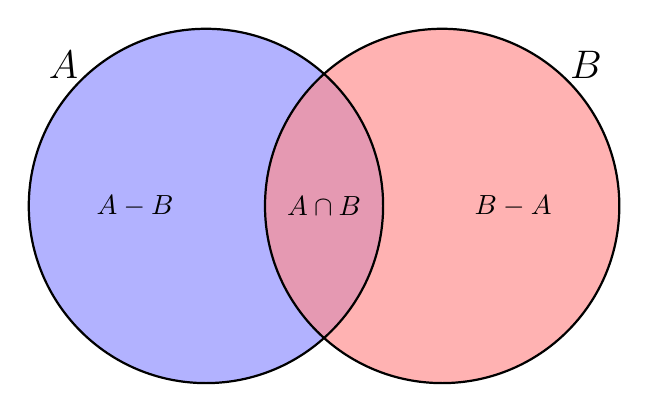
\begin{tikzpicture}[scale=1.5]
    % Define colors
    \colorlet{colorA}{blue!30}
    \colorlet{colorB}{red!30}
    \colorlet{colorInt}{purple!40}

    % Draw sets
    \begin{scope}
        \clip (0,0) circle (1.5cm);
        \fill[colorA] (-2,-2) rectangle (2,2);
        \clip (2,0) circle (1.5cm);
        \fill[colorInt] (-2,-2) rectangle (4,2);
    \end{scope}
    
    \begin{scope}
        \clip (2,0) circle (1.5cm);
        \fill[colorB] (-2,-2) rectangle (4,2);
        \clip (0,0) circle (1.5cm);
        \fill[colorInt] (-2,-2) rectangle (4,2);
    \end{scope}

    % Outlines
    \draw[thick] (0,0) circle (1.5cm);
    \draw[thick] (2,0) circle (1.5cm);

    % Labels
    \node at (-0.6, 0) {\textbf{$A - B$}};
    \node at (2.6, 0) {\textbf{$B - A$}};
    \node at (1, 0) {\textbf{$A \cap B$}};
    
    \node[above left] at (-1.0, 1.0) {\Large $A$};
    \node[above right] at (3.0, 1.0) {\Large $B$};
\end{tikzpicture}
\end{center}

\subsection{Heuristics \& "Cheats"}
\begin{itemize}
    \item \textbf{The "Let $x \in \dots$" Reflex:} Whenever you see "Prove $A \subseteq B$", your immediate, reflexive first line of the proof should be "Let $x \in A$."
    \item \textbf{Translating to Logic:} If you are stuck on a set theory proof, translate everything to propositional logic. Replace $\cup$ with $\lor$, $\cap$ with $\land$, and $\subseteq$ with $\implies$. Solve the logic puzzle, then translate back to sets.
\end{itemize}

\subsection{Pitfalls \& Fallacies}
\begin{itemize}
    \item \textbf{The Empty Set Trap:} Never write "Let $x \in A$" if there is a possibility that $A = \emptyset$. Always handle the empty set as a separate case or use contradiction.
    \item \textbf{Converse Error in Subsets:} Proving $x \in B \implies x \in A$ proves $B \subseteq A$, not $A \subseteq B$. Directionality is paramount.
    \item \textbf{Confusing Elements with Subsets:} $x \in A$ means $x$ is an element. $\{x\} \subseteq A$ means the set containing $x$ is a subset. Do not write $x \subseteq A$ unless $x$ itself is a set.
\end{itemize}

\newpage
% ==========================================
% PART 5: Conceptual Synthesis
% ==========================================
\section{Part 5: Conceptual Synthesis and The "Big Picture"}

\subsection{A) Thematic Connections}
The core theme of this chapter is \textbf{formalizing collections and their relations through rigorous logic}. In previous chapters, logic was applied to static statements (e.g., "If $n$ is even, $n^2$ is even"). Here, logic is elevated to operate on \textit{spaces} and \textit{structures}. Set theory acts as the universal translator of mathematics. By proving that $A \cap B = A \iff A \subseteq B$, we are establishing an isomorphism between algebraic operations on sets (intersection) and relational structures (subsets). 

\subsection{B) Forward and Backward Links}
\begin{itemize}
    \item \textbf{Backward Links:} This topic relies heavily on the propositional logic and proof techniques (direct, contrapositive) established in Chapters 1-3. The modular arithmetic problems explicitly link set definitions to the divisibility theorems proven in Chapter 4.1-4.2.
    \item \textbf{Forward Links:} Understanding set operations is the absolute prerequisite for \textbf{Measure Theory} and \textbf{Probability}. In advanced probability, a sample space $\Omega$ is a set. Events are subsets. A $\sigma$-algebra is a set of sets closed under countable unions and complements. Without mastering double inclusion and De Morgan's laws, defining a probability measure $\mathbb{P}: \mathcal{F} \to [0,1]$ is impossible. Furthermore, set theory leads directly into Topology (open/closed sets) and Abstract Algebra (cosets, ideals).
\end{itemize}

% ==========================================
% PART 6: Abstract Real-World Modeling
% ==========================================
\section{Part 6: Abstract Real-World Modeling (AI, ML, \& Quant Finance)}

\subsection{A) Concrete Scenarios}
\begin{enumerate}
    \item \textbf{Quantitative Finance (Derivative Pricing):} In Stochastic Calculus, the price of an asset is modeled as a stochastic process on a probability space $(\Omega, \mathcal{F}, \mathbb{P})$. Exotic options, like Double Barrier Knock-Out options, only pay out if the asset price stays within a specific channel. The event of a payout is defined strictly using set intersections and unions of hitting times.
    \item \textbf{Machine Learning (Statistical Learning Theory):} In binary classification, a model attempts to learn a decision boundary. The true positive region is a set $A$, and the predicted positive region is a set $B$. The model's loss function is often proportional to the measure of the symmetric difference $(A - B) \cup (B - A)$, which represents the classification errors.
\end{enumerate}

\subsection{B) Model Problem Setup: Probability Spaces in Algorithmic Trading}
Let us rigorously model a simplified algorithmic trading scenario using set theory and measure theory.

\textbf{The State Space:} Let $\Omega$ be the set of all possible continuous price paths of a stock over the time interval $[0, T]$. An individual path is $\omega \in \Omega$.
Let $S_t(\omega)$ be the price of the stock at time $t$. We assume $S_t$ follows a Geometric Brownian Motion governed by the Stochastic Differential Equation (SDE):
\[ dS_t = \mu S_t \, dt + \sigma S_t \, dW_t \]
where $W_t$ is a standard Brownian motion under the physical measure $\mathbb{P}$.

\textbf{Defining Events via Sets:}
An algorithmic trading strategy executes a "buy" if the stock drops below a threshold $L$, and a "sell" if it exceeds a threshold $H$. We define the hitting times:
\[ \tau_L = \inf \{ t \in [0, T] : S_t \le L \} \]
\[ \tau_H = \inf \{ t \in [0, T] : S_t \ge H \} \]

We define the following sets (events) in our $\sigma$-algebra $\mathcal{F}$:
\begin{itemize}
    \item $A = \{ \omega \in \Omega : \tau_L(\omega) \le T \}$ (The event the stock hits the lower bound).
    \item $B = \{ \omega \in \Omega : \tau_H(\omega) \le T \}$ (The event the stock hits the upper bound).
\end{itemize}

\textbf{The Optimization Problem:}
The algorithm's success relies on the stock hitting the lower bound \textit{before} hitting the upper bound, and eventually hitting the upper bound. We define this success set $C$:
\[ C = \{ \omega \in \Omega : \tau_L(\omega) < \tau_H(\omega) \} \cap B \]
To evaluate the expected return of this strategy, a quantitative researcher must compute the probability measure of this set, $\mathbb{P}(C)$, often requiring a change of measure via Girsanov's Theorem to a risk-neutral measure $\mathbb{Q}$, transforming the set-theoretic definition into a computable martingale problem.

\newpage
% ==========================================
% PART 7: Common Variations and Untested Concepts
% ==========================================
\section{Part 7: Common Variations and Untested Concepts}

A standard university curriculum in abstract mathematics usually includes proofs involving \textbf{Power Sets} and \textbf{Arbitrary (Infinite) Unions/Intersections}, which were not explicitly tested in the provided homework selection.

\subsection{Missing Concept 1: Power Sets}
\begin{definition}
The power set of $A$, denoted $\mathcal{P}(A)$, is the set of all subsets of $A$. Formally, $\mathcal{P}(A) = \{X : X \subseteq A\}$.
\end{definition}

\begin{theorem}
For any sets $A$ and $B$, $A \subseteq B \iff \mathcal{P}(A) \subseteq \mathcal{P}(B)$.
\end{theorem}
\begin{proof}
\textbf{($\implies$):} Assume $A \subseteq B$. Let $X \in \mathcal{P}(A)$. By definition of the power set, $X \subseteq A$. Since subset inclusion is transitive (if $X \subseteq A$ and $A \subseteq B$, then $X \subseteq B$), it follows that $X \subseteq B$. Therefore, $X \in \mathcal{P}(B)$. Thus, $\mathcal{P}(A) \subseteq \mathcal{P}(B)$.

\textbf{($\impliedby$):} Assume $\mathcal{P}(A) \subseteq \mathcal{P}(B)$. We know that every set is a subset of itself, so $A \subseteq A$, which means $A \in \mathcal{P}(A)$. Since $\mathcal{P}(A) \subseteq \mathcal{P}(B)$, it follows that $A \in \mathcal{P}(B)$. By definition of the power set, this means $A \subseteq B$.
\end{proof}

\subsection{Missing Concept 2: Generalized De Morgan's Laws}
In measure theory, we deal with countably infinite unions of sets.
\begin{theorem}
Let $\{A_i\}_{i \in I}$ be an indexed family of sets. Then $\overline{\bigcup_{i \in I} A_i} = \bigcap_{i \in I} \overline{A_i}$.
\end{theorem}
\begin{proof}
Let $x \in \overline{\bigcup_{i \in I} A_i}$. This means $x \notin \bigcup_{i \in I} A_i$. 
By definition of union, it is false that there exists an $i \in I$ such that $x \in A_i$. 
Therefore, for all $i \in I$, $x \notin A_i$. 
This means that for all $i \in I$, $x \in \overline{A_i}$. 
By definition of intersection, $x \in \bigcap_{i \in I} \overline{A_i}$. 
The steps are perfectly reversible, establishing equality.
\end{proof}

\newpage
% ==========================================
% PART 8: Advanced Diagnostic Testing
% ==========================================
\section{Part 8: Advanced Diagnostic Testing: "Find the Flaw"}

Below are five proofs that appear rigorous but contain a single, critical logical or mathematical flaw. Your task as the grader is to identify the flaw and provide the correct logical step.

\subsection{Flawed Proof 1}
\textbf{Claim:} For any sets $A$ and $B$, if $A \cup B = B$, then $A \subseteq B$.
\begin{proof}
Assume $A \cup B = B$. We want to show $A \subseteq B$. Let $x \in B$. Since $A \cup B = B$, we can substitute $B$ to get $x \in A \cup B$. By definition of union, $x \in A$ or $x \in B$. Since this implies $x$ can be in $A$, we have shown that elements of $B$ are in $A$, and thus $A \subseteq B$. $\blacksquare$
\end{proof}

\subsection{Flawed Proof 2}
\textbf{Claim:} For any sets $A, B,$ and $C$, $A - (B \cup C) = (A - B) \cup (A - C)$.
\begin{proof}
Let $x \in A - (B \cup C)$. By definition, $x \in A$ and $x \notin (B \cup C)$. 
By De Morgan's Laws, $x \notin (B \cup C)$ means $x \notin B$ and $x \notin C$. 
Since $x \in A$, we can distribute this to say $(x \in A \land x \notin B)$ and $(x \in A \land x \notin C)$. 
This means $x \in (A - B)$ and $x \in (A - C)$. 
Therefore, $x \in (A - B) \cup (A - C)$. $\blacksquare$
\end{proof}

\subsection{Flawed Proof 3}
\textbf{Claim:} If $A \cap B = \emptyset$, then $A = \emptyset$ or $B = \emptyset$.
\begin{proof}
We proceed by contradiction. Assume $A \cap B = \emptyset$, but $A \neq \emptyset$ and $B \neq \emptyset$. 
Since $A \neq \emptyset$, there exists some element $x \in A$. 
Since $B \neq \emptyset$, there exists some element $x \in B$. 
Therefore, $x \in A$ and $x \in B$, which means $x \in A \cap B$. 
This contradicts the premise that $A \cap B = \emptyset$. Thus, $A = \emptyset$ or $B = \emptyset$. $\blacksquare$
\end{proof}

\subsection{Flawed Proof 4}
\textbf{Claim:} For any set $A$, $\emptyset \subseteq A$.
\begin{proof}
To prove $\emptyset \subseteq A$, we must show that for all $x$, if $x \in \emptyset$, then $x \in A$. 
Let $x \in \emptyset$. Since $x$ is in the empty set, and the empty set is a subset of every set, $x$ must also be in $A$. Therefore, $\emptyset \subseteq A$. $\blacksquare$
\end{proof}

\subsection{Flawed Proof 5}
\textbf{Claim:} Let $A$ and $B$ be sets. If $\mathcal{P}(A) \subseteq \mathcal{P}(B)$, then $A \subseteq B$.
\begin{proof}
Assume $\mathcal{P}(A) \subseteq \mathcal{P}(B)$. Let $x \in A$. 
Since $x \in A$, it follows that $x \in \mathcal{P}(A)$. 
Because $\mathcal{P}(A) \subseteq \mathcal{P}(B)$, we deduce that $x \in \mathcal{P}(B)$. 
By definition of the power set, this means $x \in B$. 
Therefore, $A \subseteq B$. $\blacksquare$
\end{proof}

\vspace{1cm}
\hrule
\vspace{0.5cm}
\subsection*{Solution Key: Resolutions to the Flaws}
\begin{itemize}
    \item \textbf{Flaw 1:} \textit{Converse Error.} The proof starts with "Let $x \in B$". To prove $A \subseteq B$, one MUST start with "Let $x \in A$". The correct step: Let $x \in A$. Then $x \in A \cup B$. Since $A \cup B = B$, $x \in B$. Thus $A \subseteq B$.
    \item \textbf{Flaw 2:} \textit{Logical Translation Error.} The proof correctly deduces $x \in (A - B)$ \textbf{AND} $x \in (A - C)$. However, it then incorrectly translates the logical AND ($\land$) into a set UNION ($\cup$). It should translate to an INTERSECTION ($\cap$). The true identity is $A - (B \cup C) = (A - B) \cap (A - C)$.
    \item \textbf{Flaw 3:} \textit{Variable Re-use Fallacy.} The proof assumes that because $A$ is non-empty, it has an element $x$, and because $B$ is non-empty, it has an element $x$. It incorrectly uses the \textit{same} variable $x$ for both sets. $A$ might contain $y$ and $B$ might contain $z$, where $y \neq z$. The claim itself is mathematically false (e.g., $A=\{1\}, B=\{2\}$).
    \item \textbf{Flaw 4:} \textit{Circular Reasoning.} The proof attempts to prove that the empty set is a subset of $A$ by stating "the empty set is a subset of every set" in the middle of the deduction. The correct proof uses vacuous truth: The statement "If $x \in \emptyset$, then $x \in A$" is vacuously true because the hypothesis $x \in \emptyset$ is always false.
    \item \textbf{Flaw 5:} \textit{Element vs. Subset Confusion.} The proof states "Since $x \in A$, it follows that $x \in \mathcal{P}(A)$." This is false. The elements of a power set are \textit{sets}. The correct statement is $\{x\} \subseteq A$, which implies $\{x\} \in \mathcal{P}(A)$. Then $\{x\} \in \mathcal{P}(B) \implies \{x\} \subseteq B \implies x \in B$.
\end{itemize}

\end{document}